\documentclass[UTF8,a4paper,zihao=-4,fontset=fandol]{ctexart}

\usepackage[left=2.5cm,right=2.5cm,top=2.5cm,bottom=2.5cm]{geometry}
\usepackage{amsmath,amssymb,bm}
\usepackage{booktabs,longtable,tabularx,array,multirow}
\usepackage{graphicx,float,caption,subcaption}
\usepackage{xcolor}
\usepackage{fancyhdr}
\usepackage{enumitem}
\usepackage{hyperref}
\usepackage{setspace}
\usepackage{titlesec}

\hypersetup{colorlinks=true,linkcolor=black,citecolor=black,urlcolor=blue,breaklinks=true}
\graphicspath{{../../outputs/figures/}}
\setlength{\parindent}{2em}
\setlength{\parskip}{0pt}
\linespread{1.22}
\captionsetup{font=small,labelsep=quad}
\setlist{nosep,leftmargin=2em}
\titleformat{\section}{\centering\heiti\zihao{4}}{\thesection}{1em}{}
\titleformat{\subsection}{\heiti\zihao{-4}}{\thesubsection}{0.8em}{}
\pagestyle{fancy}
\fancyhf{}
\fancyfoot[C]{\thepage}
\renewcommand{\headrulewidth}{0pt}
\newcolumntype{C}[1]{>{\centering\arraybackslash}p{#1}}
\newcolumntype{L}[1]{>{\raggedright\arraybackslash}p{#1}}
\newcommand{\unit}[1]{\,\mathrm{#1}}
\newcommand{\dif}{\mathop{}\!\mathrm{d}}

\begin{document}

\pagenumbering{Roman}
\thispagestyle{empty}
\begin{center}
  {\heiti\zihao{2} 基于守恒有限体积法的圆柱药材热湿传递与收缩干燥模型}
\end{center}

\vspace{0.8em}
\noindent{\heiti\zihao{4} 摘\quad 要：}
热风干燥中，药材内部温度和水分的径向迁移决定了升温速度与最终达标时刻。本文将圆柱药材简化为一维轴对称径向区域，建立热传导方程与非线性水分扩散方程；表面采用第三类换热、传质边界，烘房实测序列用分段线性插值描述。问题 1 采用常热物性和浓度相关扩散系数；问题 2、3 引入随水分浓度和温度变化的物性关联式；问题 4 令 $\xi=r/R(t)$ 为随收缩运动的无量纲物质坐标，并由附件 2 插值得到半径路径。空间上采用节点中心守恒有限体积法，时间上使用 BDF 法求解半离散刚性系统；另以队友独立实现的全隐式有限体积法交叉复核。

计算表明：预热 $1800\unit{s}$ 后，药材中心与表面温度分别为 $33.5753\,^{\circ}\mathrm{C}$ 和 $36.7856\,^{\circ}\mathrm{C}$，相应干基含水率为 $2.5500\unit{kg/kg}$ 和 $1.5102\unit{kg/kg}$。采用附录 3 物性且半径固定时，两套求解器给出的达标时间为 $57.16\sim57.21\unit{h}$，故报告为约 $57.2\unit{h}$；采用附录 4 物性与实测收缩路径时为 $50.82\sim50.86\unit{h}$，即约 $50.9\unit{h}$，结束半径约 $1.200\unit{cm}$。在同一物性参数下的反事实计算表明，收缩路径可显著缩短模型内扩散时间，但幅度依赖均匀收缩假设。BDF 事件根在容差与步长收紧后变化不超过 $4.5\unit{s}$；末值保持、末段均值和平滑渐近三种炉况延拓的时长差异约 $0.5\%$。扩散系数的前因子和两个指数项是主导不确定性。主模型未显式耦合蒸发潜热：量级审计说明题给热、质边界尚不足以闭合潜热反馈，因此温度结果应理解为题给等效边界下的条件预测。

\vspace{0.6em}
\noindent{\heiti 关键词：}圆柱干燥；热湿传递；有限体积法；移动边界；BDF；灵敏度分析

\newpage
\pagenumbering{arabic}

\section{问题重述与分析}

\subsection{问题重述}

研究对象为长 $25\unit{cm}$、初始半径 $2\unit{cm}$ 的近似圆柱形中药材。初始温度为 $28\,^{\circ}\mathrm{C}$，初始水分浓度（干基含水率）为 $2.55\unit{kg/kg}$。题目要求根据烘房温度和空气水分浓度序列，依次求解以下四项任务：建立预热阶段的温度场和水分场；使用附录 3 的变物性经验式描述前 $3\unit{h}$ 的完整烘干过程；确定固定半径条件下各处水分浓度低于 $0.15\unit{kg/kg}$ 的首次时刻；最后根据附件 2 的半径变化数据和附录 4 的物性式建立收缩域模型，重新计算烘干时长。

完整结果还须分别按 $1\unit{s}$ 或 $60\unit{s}$ 的时间间隔、$0.1\unit{cm}$ 的空间间隔写入四个指定 Excel 文件。因而模型不仅要给出若干观测点的数值，还应在长时间、强非线性和移动边界条件下保持稳定，并能准确识别阈值事件。

\subsection{问题分析}

圆柱的几何细长程度及端部面积占比满足
\begin{equation}
\frac{L}{2R_0}=6.25,\qquad
\frac{2\pi R_0^2}{2\pi R_0L}=\frac{R_0}{L}=0.08.
\end{equation}
结合题目只要求到中心的径向距离，主模型先忽略端部影响，将其视为轴对称长圆柱，以径向坐标 $r$ 描述场变量；端部近似的适用边界在模型局限中说明。

温度通过导热与表面对流换热变化，水分通过内部扩散与表面对流传质变化。问题 2 以后，密度、比热、导热系数和扩散系数均随状态改变，使半离散系统呈刚性。问题 4 又引入 $R(t)$，若直接在物理坐标上重构网格会造成插值误差，故采用固定的物质坐标 $\xi=r/R(t)$。

四问构成逐层递进的模型链：问题 1 用常热物性和浓度相关扩散系数检验基础方程和边界实现；问题 2 检验时变炉况与非线性物性；问题 3 在同一固定域上进行阈值事件检测；问题 4 改变为收缩域。为避免混淆，本文另设同物性参数下的固定半径/收缩半径反事实，而不把问题 3、4 的时间差直接归结为尺寸变化。

\section{模型假设}

结合题目信息和数值可识别性，作如下假设：

\begin{enumerate}
  \item 药材在任一横截面上轴对称，轴向梯度和两端传热传质可以忽略，场变量仅依赖 $r$ 与 $t$。
  \item 药材内部不存在体热源与水分源；水分浓度是题目定义的干基含水率，其扩散由 Fick 型方程描述。
  \item 药材表面与热风之间分别满足对流换热和对流传质边界。题目对问题 2--4 未另给 $h$ 与 $h_m$，故沿用附录 2 数值，并在灵敏度分析中检查其影响。
  \item 附件 1、2 的离散序列在观测点之间分段线性变化。附件 1 在 $14400\unit{s}$ 后缺少炉况记录，基线情形维持末次观测值不变，并以末段均值保持和平滑渐近作对照。
  \item 问题 4 的收缩在径向上均匀发生，长度维持 $25\unit{cm}$；$\xi$ 标记随收缩运动的物质点。该假设省略了显式的收缩速度项与体积稀释项，是对题给半径数据的工程化闭合。
  \item 主模型把题给热、质边界视为分别标定的等效闭合，不向能量方程机械叠加蒸发潜热项。这并非假定潜热很小；题目未给干物质密度、气固平衡含水率关系与有效汽化潜热，直接耦合会造成量纲口径和能量供需不一致。本文另作量级审计，并将正确耦合形式列为扩展模型。
\end{enumerate}

\section{符号说明}

\begin{table}[H]
\centering
\caption*{主要符号与单位}
\begin{tabular}{C{2.0cm}L{7.4cm}C{3.0cm}}
\toprule
符号 & 含义 & 单位 \\
\midrule
$r$ & 到药材中心轴的径向距离 & $\mathrm{m}$ \\
$R(t)$ & 药材瞬时半径 & $\mathrm{m}$ \\
$\xi$ & 无量纲物质坐标，$\xi=r/R(t)$ & $1$ \\
$t$ & 烘干时间 & $\mathrm{s}$ \\
$T,T_\infty$ & 药材温度、烘房温度 & $^{\circ}\mathrm{C}$ 或 $\mathrm{K}$ \\
$C,C_\infty$ & 药材水分浓度、空气水分浓度 & $\mathrm{kg/kg}$ \\
$\rho$ & 药材密度 & $\mathrm{kg/m^3}$ \\
$\rho_d$ & 单位当前体积内的干物质质量（审计量） & $\mathrm{kg/m^3}$ \\
$c_p$ & 定压比热容 & $\mathrm{J/(kg\cdot K)}$ \\
$k$ & 导热系数 & $\mathrm{W/(m\cdot K)}$ \\
$D$ & 水分扩散系数 & $\mathrm{m^2/s}$ \\
$h$ & 对流换热系数 & $\mathrm{W/(m^2\cdot K)}$ \\
$h_m$ & 对流传质系数 & $\mathrm{m/s}$ \\
$L_v$ & 水的有效汽化潜热（审计参数） & $\mathrm{J/kg}$ \\
\bottomrule
\end{tabular}
\end{table}

\section{统一热湿传递模型}

\subsection{控制方程}

圆柱坐标下的径向导热和扩散方程分别为\cite{bergman2018,crank1975}

\begin{equation}
\rho(C)c_p(C)\frac{\partial T}{\partial t}
=\frac{1}{r}\frac{\partial}{\partial r}
\left[rk(C)\frac{\partial T}{\partial r}\right],
\label{eq:heat}
\end{equation}

\begin{equation}
\frac{\partial C}{\partial t}
=\frac{1}{r}\frac{\partial}{\partial r}
\left[rD(C,T_K)\frac{\partial C}{\partial r}\right],
\label{eq:mass}
\end{equation}
其中 $T_K=T+273.15$。初始条件为
\begin{equation}
T(r,0)=28\,^{\circ}\mathrm{C},\qquad C(r,0)=2.55\unit{kg/kg}.
\label{eq:initial}
\end{equation}

圆柱中心满足对称条件
\begin{equation}
\left.\frac{\partial T}{\partial r}\right|_{r=0}=0,
\qquad
\left.\frac{\partial C}{\partial r}\right|_{r=0}=0.
\label{eq:center_bc}
\end{equation}
表面采用第三类边界条件
\begin{equation}
k\left.\frac{\partial T}{\partial r}\right|_{r=R}
=h\,[T_\infty(t)-T(R,t)],
\label{eq:heat_bc}
\end{equation}
\begin{equation}
D\left.\frac{\partial C}{\partial r}\right|_{r=R}
=h_m\,[C_\infty(t)-C(R,t)].
\label{eq:mass_bc}
\end{equation}
式中符号方向取径向向外，右端为进入药材的通量；干燥时 $C_\infty<C(R,t)$，故式\eqref{eq:mass_bc}给出负的水分通量。

\subsection{外部边界与物性参数}

附件 1 的 $T_\infty(t)$ 和 $C_\infty(t)$ 采用分段线性插值。其记录范围为 $0\sim14400\unit{s}$；长期计算采用常值延拓
\begin{equation}
T_\infty(t)=50.165\,^{\circ}\mathrm{C},\qquad
C_\infty(t)=0.04986\unit{kg/kg},\qquad t>14400\unit{s}.
\label{eq:air_extension}
\end{equation}
所有问题使用
\begin{equation}
h=25\unit{W/(m^2\cdot K)},\qquad h_m=8\times10^{-7}\unit{m/s}.
\label{eq:boundary_coeff}
\end{equation}
图\ref{fig:inputs}给出两组原始边界输入。温度较早接近平台，但温度与空气水分浓度约在 $2.5\unit{h}$ 后才同时进入末段窄幅波动带，故图中将其称为“超稳段”。半径在约 $20\unit{h}$ 后接近平台，而附件 1 只覆盖前 $4\unit{h}$，这一时间覆盖差异是长期预测的主要外部不确定性来源。

\begin{figure}[H]
\centering
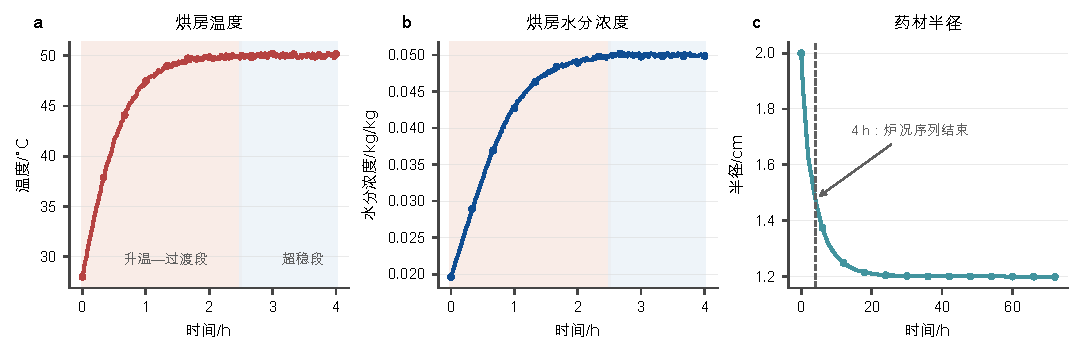
\includegraphics[width=\textwidth]{problem_a_figure_04_boundary_and_radius_v03.pdf}
\caption{烘房边界条件与药材半径输入。圆点为抽样显示的附件观测，曲线为分段线性插值；约 $2.5\unit{h}$ 后温湿边界同时进入超稳段。}
\label{fig:inputs}
\end{figure}

问题 1 使用常参数 $\rho=820\unit{kg/m^3}$、$c_p=2600\unit{J/(kg\cdot K)}$、$k=0.36\unit{W/(m\cdot K)}$，并令
\begin{equation}
D(C)=7\times10^{-9}\exp\left(-\frac{0.89}{C}\right).
\label{eq:q1_D}
\end{equation}

问题 2、3 使用附录 3 关联式
\begin{equation}
\begin{aligned}
\rho&=650+128C,\\
c_p&=1450+2736\frac{C}{C+1},\\
k&=0.21+0.38\frac{C}{C+1},\\
D&=2.4\times10^{-3}
\exp\left(-\frac{0.45}{C}\right)
\exp\left(-\frac{3850}{T_K}\right).
\end{aligned}
\label{eq:appendix3}
\end{equation}

问题 4 使用附录 4 关联式
\begin{equation}
\begin{aligned}
\rho&=760+90C,\\
c_p&=1850+2150\frac{C}{C+1},\\
k&=0.12+0.20\frac{C}{C+1},\\
D&=4.2\times10^{-4}
\exp\left(-\frac{0.30}{C}\right)
\exp\left(-\frac{3850}{T_K}\right).
\end{aligned}
\label{eq:appendix4}
\end{equation}

\subsection{收缩域坐标变换}

问题 4 由附件 2 插值得到 $R(t)$，并定义
\begin{equation}
\xi=\frac{r}{R(t)},\qquad 0\le\xi\le1.
\label{eq:xi}
\end{equation}
在均匀径向收缩、$\xi$ 随物质点运动的假设下，模型写为
\begin{equation}
\rho c_p\left.\frac{\partial T}{\partial t}\right|_{\xi}
=\frac{1}{\xi R(t)^2}\frac{\partial}{\partial\xi}
\left(\xi k\frac{\partial T}{\partial\xi}\right),
\label{eq:moving_heat}
\end{equation}
\begin{equation}
\left.\frac{\partial C}{\partial t}\right|_{\xi}
=\frac{1}{\xi R(t)^2}\frac{\partial}{\partial\xi}
\left(\xi D\frac{\partial C}{\partial\xi}\right).
\label{eq:moving_mass}
\end{equation}
相应表面条件中的物理梯度满足 $\partial/\partial r=R(t)^{-1}\partial/\partial\xi$。为避免法向与热流正方向混淆，令向外热流和水分流分别为 $q_n=-k\partial T/\partial r$、$j_n=-D\partial C/\partial r$，则在 $\xi=1$ 处有
\begin{equation}
q_n=h(T_s-T_\infty),\qquad j_n=h_m(C_s-C_\infty),
\label{eq:moving_flux_bc}
\end{equation}
等价地，
\begin{equation}
\frac{k}{R(t)}\left.\frac{\partial T}{\partial\xi}\right|_{\xi=1}
=h(T_\infty-T_s),\qquad
\frac{D}{R(t)}\left.\frac{\partial C}{\partial\xi}\right|_{\xi=1}
=h_m(C_\infty-C_s).
\label{eq:moving_gradient_bc}
\end{equation}
这一处理把移动边界固定到 $\xi=1$，避免每个时间步重新划分网格。由于题目没有给出局部固体速度、孔隙率和干物质密度，式\eqref{eq:moving_mass}应理解为基于物质坐标的等效扩散闭合，而非完整的变形多孔介质守恒模型。

\section{数值方法}

\subsection{守恒有限体积离散}

将区间 $[0,R]$ 划分为 $N$ 个等长区间并在节点 $r_i$ 存储未知量。第 $i$ 个控制体的径向面积权重为
\begin{equation}
V_i^{\ast}=\frac{r_{i+1/2}^2-r_{i-1/2}^2}{2}.
\label{eq:volume}
\end{equation}
对一般扩散方程
\begin{equation}
\frac{\partial u}{\partial t}
=\frac{1}{r}\frac{\partial}{\partial r}
\left(r\Gamma\frac{\partial u}{\partial r}\right)
\end{equation}
积分后得到守恒半离散式\cite{patankar1980}
\begin{equation}
V_i^{\ast}\frac{\dif u_i}{\dif t}
=r_{i+1/2}\Gamma_{i+1/2}\frac{u_{i+1}-u_i}{\Delta r}
-r_{i-1/2}\Gamma_{i-1/2}\frac{u_i-u_{i-1}}{\Delta r}.
\label{eq:fvm}
\end{equation}
温度方程右端再除以 $\rho_i c_{p,i}$，水分方程直接使用式\eqref{eq:fvm}。生产计算采用算术平均
\begin{equation}
\Gamma_{i+1/2}=\frac{\Gamma_i+\Gamma_{i+1}}{2},
\label{eq:hmean}
\end{equation}
并以调和平均作为独立离散对照；网格加密后两者收敛到同一结果。中心面通量置零，表面面通量直接由式\eqref{eq:heat_bc}和式\eqref{eq:mass_bc}给出，因此每个控制体的变化均来自相邻面通量差。

\subsection{时间积分与事件判定}

半离散后得到 $2(N+1)$ 维刚性常微分方程组。采用隐式 BDF 方法积分\cite{hairer1996}，并提供块三对角 Jacobian 稀疏结构。正式计算中相对容差为 $2\times10^{-7}$；温度、水分绝对容差分别为 $10^{-8}$ 和 $10^{-9}$，且限制内部最大步长不超过 $60\unit{s}$。附件观测点处保留分段插值折点，避免积分跨越边界突变。实现基于 SciPy 的初值问题求解器\cite{virtanen2020}。

理论达标时刻定义为
\begin{equation}
t_{\mathrm{dry}}=\inf\left\{t:\max_{0\le r\le R(t)}C(r,t)<0.15\right\}.
\label{eq:drytime}
\end{equation}
数值序列中最大值始终位于中心。本文将事件函数 $g(t)=C(0,t)-0.15$ 直接交给 BDF 求解器作根定位，而不再用相邻 $60\unit{s}$ 输出点线性插值。官方文件按四位小数显示；为保证离散误差计入后仍严格显示为 $0.1499$，采用
\begin{equation}
C_{\max}^{(N)}(t)+\varepsilon_C<0.14995,
\qquad \varepsilon_C=3.0\times10^{-5},
\label{eq:display_safe}
\end{equation}
并将首次满足该式的时刻向上取整到下一完整 $60\unit{s}$。其中 $\varepsilon_C$ 大于当前两级网格在关键时刻的最大差。连续事件时长用于模型解释，保守时长用于 Excel 最后一行。

\section{问题 1：预热阶段}

问题 1 在固定半径 $R=2\unit{cm}$ 上使用式\eqref{eq:q1_D}与常热物性。内部网格取 $N=2560$，每 $1\unit{s}$ 输出一次，并插值得到每隔 $0.1\unit{cm}$ 的结果。图\ref{fig:q1profiles}显示，温度从表面向中心传播，而水分由表层先行逸出；在前 $1800\unit{s}$ 内，水分前沿尚未使中心发生可见变化。代表性节点值见表\ref{tab:q1temperature}和表\ref{tab:q1moisture}。

\begin{figure}[H]
\centering
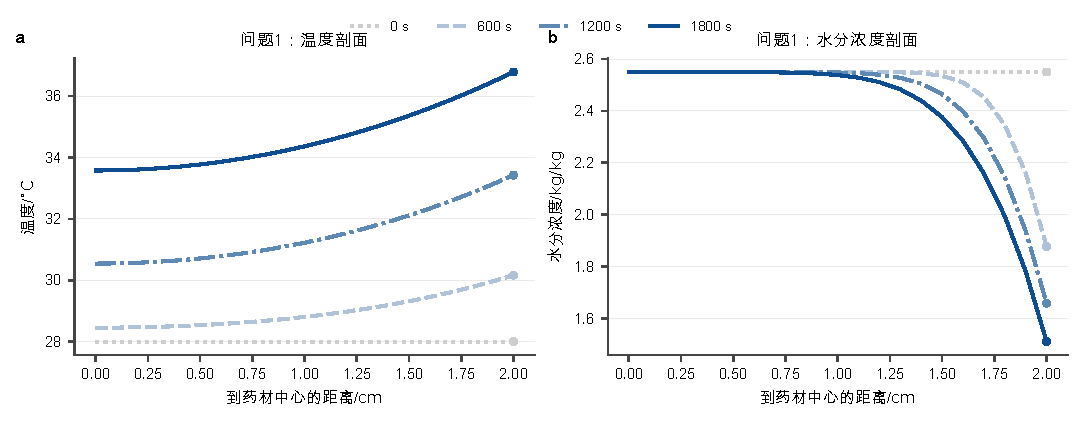
\includegraphics[width=\textwidth]{problem_a_figure_05_preheat_profiles_cn_v03.pdf}
\caption{问题 1 的温度与水分浓度径向剖面。$0\unit{s}$ 曲线由初始条件给出。}
\label{fig:q1profiles}
\end{figure}

\begin{table}[H]
\centering
\caption{$30\unit{min}$ 内药材的温度（$^{\circ}\mathrm{C}$）}
\label{tab:q1temperature}
\small
\begin{tabular}{rrrrrr}
\toprule
时间/$\mathrm{s}$ & $0\unit{cm}$ & $0.5\unit{cm}$ & $1.0\unit{cm}$ & $1.5\unit{cm}$ & $2.0\unit{cm}$ \\
\midrule
100  & 28.0001 & 28.0003 & 28.0040 & 28.0327 & 28.1801 \\
300  & 28.0408 & 28.0635 & 28.1514 & 28.3681 & 28.8488 \\
600  & 28.4533 & 28.5360 & 28.8039 & 29.3159 & 30.1652 \\
900  & 29.3243 & 29.4583 & 29.8755 & 30.6161 & 31.7304 \\
1200 & 30.5427 & 30.7098 & 31.2223 & 32.1126 & 33.4276 \\
1500 & 31.9957 & 32.1867 & 32.7660 & 33.7463 & 35.1203 \\
1800 & 33.5753 & 33.7720 & 34.3642 & 35.3621 & 36.7856 \\
\bottomrule
\end{tabular}
\end{table}

\begin{table}[H]
\centering
\caption{$30\unit{min}$ 内药材的水分浓度（$\mathrm{kg/kg}$）}
\label{tab:q1moisture}
\small
\begin{tabular}{rrrrrr}
\toprule
时间/$\mathrm{s}$ & $0\unit{cm}$ & $0.5\unit{cm}$ & $1.0\unit{cm}$ & $1.5\unit{cm}$ & $2.0\unit{cm}$ \\
\midrule
100  & 2.5500 & 2.5500 & 2.5500 & 2.5500 & 2.2470 \\
300  & 2.5500 & 2.5500 & 2.5500 & 2.5492 & 2.0508 \\
600  & 2.5500 & 2.5500 & 2.5500 & 2.5353 & 1.8770 \\
900  & 2.5500 & 2.5500 & 2.5497 & 2.5045 & 1.7547 \\
1200 & 2.5500 & 2.5500 & 2.5482 & 2.4646 & 1.6586 \\
1500 & 2.5500 & 2.5499 & 2.5445 & 2.4206 & 1.5787 \\
1800 & 2.5500 & 2.5497 & 2.5383 & 2.3755 & 1.5102 \\
\bottomrule
\end{tabular}
\end{table}

\section{问题 2：变物性完整烘干模型}

问题 2 用式\eqref{eq:appendix3}替换常物性，仍令 $R=2\unit{cm}$。前 $3\unit{h}$ 完全处于附件 1 的观测范围内，不涉及长期外推。正式网格取 $N=1280$。图\ref{fig:q2profiles}表明，温度场在 $3\unit{h}$ 内已接近 $50\,^{\circ}\mathrm{C}$，但水分仍保留明显径向梯度，说明后续干燥时长主要受内部传质控制；详细节点值列于表\ref{tab:q2temperature}和表\ref{tab:q2moisture}。

\begin{figure}[H]
\centering
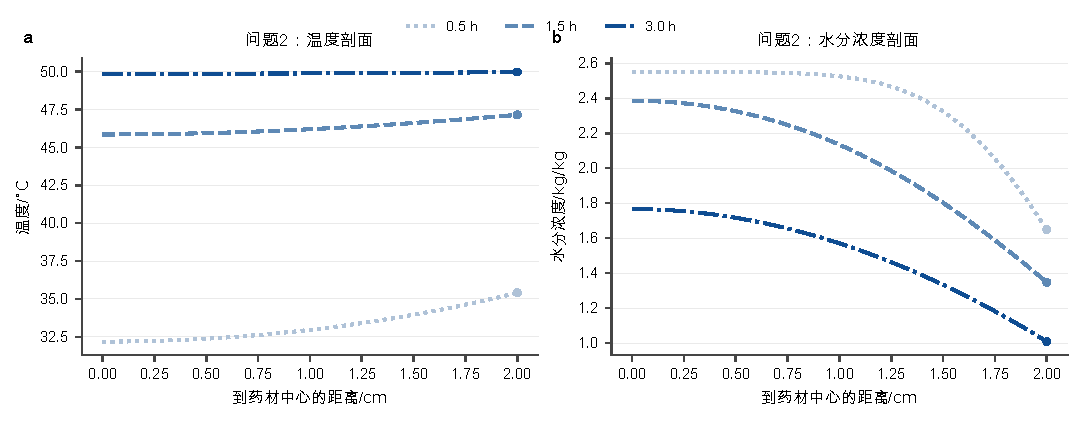
\includegraphics[width=\textwidth]{problem_a_figure_06_q2_profiles_cn_v03.pdf}
\caption{问题 2 前 $3\unit{h}$ 的温度与水分浓度径向剖面。}
\label{fig:q2profiles}
\end{figure}

\begin{table}[H]
\centering
\caption{$3\unit{h}$ 内药材的温度（$^{\circ}\mathrm{C}$）}
\label{tab:q2temperature}
\small
\begin{tabular}{rrrrrr}
\toprule
时间/$\mathrm{h}$ & $0\unit{cm}$ & $0.5\unit{cm}$ & $1.0\unit{cm}$ & $1.5\unit{cm}$ & $2.0\unit{cm}$ \\
\midrule
0.5 & 32.1893 & 32.3821 & 32.9660 & 33.9608 & 35.4131 \\
1.0 & 40.3816 & 40.5536 & 41.0605 & 41.8782 & 42.9976 \\
1.5 & 45.8468 & 45.9348 & 46.1929 & 46.6051 & 47.1400 \\
2.0 & 48.4503 & 48.4881 & 48.5985 & 48.7736 & 49.0034 \\
2.5 & 49.4670 & 49.4792 & 49.5137 & 49.5653 & 49.6609 \\
3.0 & 49.8495 & 49.8553 & 49.8746 & 49.9101 & 49.9664 \\
\bottomrule
\end{tabular}
\end{table}

\begin{table}[H]
\centering
\caption{$3\unit{h}$ 内药材的水分浓度（$\mathrm{kg/kg}$）}
\label{tab:q2moisture}
\small
\begin{tabular}{rrrrrr}
\toprule
时间/$\mathrm{h}$ & $0\unit{cm}$ & $0.5\unit{cm}$ & $1.0\unit{cm}$ & $1.5\unit{cm}$ & $2.0\unit{cm}$ \\
\midrule
0.5 & 2.5499 & 2.5489 & 2.5256 & 2.3257 & 1.6486 \\
1.0 & 2.5257 & 2.4948 & 2.3578 & 2.0230 & 1.4711 \\
1.5 & 2.3861 & 2.3256 & 2.1344 & 1.8020 & 1.3476 \\
2.0 & 2.1709 & 2.1084 & 1.9236 & 1.6259 & 1.2311 \\
2.5 & 1.9566 & 1.9006 & 1.7360 & 1.4720 & 1.1166 \\
3.0 & 1.7662 & 1.7165 & 1.5702 & 1.3333 & 1.0081 \\
\bottomrule
\end{tabular}
\end{table}

\section{问题 3：固定半径下的达标时间}

问题 3 延续式\eqref{eq:appendix3}并将附件 1 的末值按式\eqref{eq:air_extension}外推。中心水分浓度随时间单调下降，且始终为截面最大值。队友更新的全隐式有限体积解在 $N=640$ 时给出 $57.2108\unit{h}$；BDF 在 $N=2560$ 时的机器事件根为 $57.1686\unit{h}$。两套独立时间离散的差异约 $0.04\unit{h}$，大于单纯事件容差误差，故正文不把秒级机器输出当作物理精度，报告
\begin{equation}
t_{\mathrm{dry},3}\approx57.2\unit{h}\approx2.38\unit{d}.
\end{equation}
结果文件的结束行不直接取理论根，而按式\eqref{eq:display_safe}增加显示与离散双重余量。正式重算得到结束时刻 $206100\unit{s}=57.2500\unit{h}$，计算最大值为 $0.1499143\unit{kg/kg}$；加上 $\varepsilon_C$ 后为 $0.1499443\unit{kg/kg}<0.14995\unit{kg/kg}$，故四位小数显示安全成立。表\ref{tab:q3}列出关键时刻的径向分布。

\begin{table}[H]
\centering
\caption{固定半径烘干过程的水分浓度（$\mathrm{kg/kg}$）}
\label{tab:q3}
\small
\begin{tabular}{rrrrrr}
\toprule
时间/$\mathrm{h}$ & $0\unit{cm}$ & $0.5\unit{cm}$ & $1.0\unit{cm}$ & $1.5\unit{cm}$ & $2.0\unit{cm}$ \\
\midrule
6  & 1.0156 & 0.9868 & 0.9006 & 0.7546 & 0.5335 \\
12 & 0.4548 & 0.4418 & 0.4019 & 0.3289 & 0.1639 \\
18 & 0.2979 & 0.2906 & 0.2679 & 0.2247 & 0.0842 \\
24 & 0.2371 & 0.2321 & 0.2161 & 0.1851 & 0.0663 \\
30 & 0.2053 & 0.2013 & 0.1887 & 0.1637 & 0.0597 \\
36 & 0.1854 & 0.1821 & 0.1714 & 0.1501 & 0.0565 \\
42 & 0.1717 & 0.1687 & 0.1593 & 0.1404 & 0.0547 \\
48 & 0.1615 & 0.1588 & 0.1504 & 0.1332 & 0.0536 \\
54 & 0.1535 & 0.1511 & 0.1433 & 0.1275 & 0.0528 \\
57.2500 & 0.1499 & 0.1476 & 0.1401 & 0.1249 & 0.0525 \\
\bottomrule
\end{tabular}
\end{table}

\section{问题 4：考虑半径收缩的烘干时间}

问题 4 使用式\eqref{eq:appendix4}和式\eqref{eq:moving_heat}--\eqref{eq:moving_mass}。附件 2 显示半径由 $2.000\unit{cm}$ 快速减小，并在长时段接近 $1.198\unit{cm}$。队友全隐式解与 $N=2560$ 的 BDF 事件解分别为 $50.8634\unit{h}$ 与 $50.8243\unit{h}$，据其差异报告
\begin{equation}
t_{\mathrm{dry},4}\approx50.9\unit{h}\approx2.12\unit{d},
\end{equation}
此时半径约为 $1.200\unit{cm}$。提交末行取 $183180\unit{s}=50.8833\unit{h}$，其显示安全校验为
\begin{equation}
0.1498904+3\times10^{-5}=0.1499204<0.14995.
\end{equation}
因此该末行满足式\eqref{eq:display_safe}。图\ref{fig:endpoint}直观展示两问的达标前沿与收缩边界。

\begin{figure}[H]
\centering
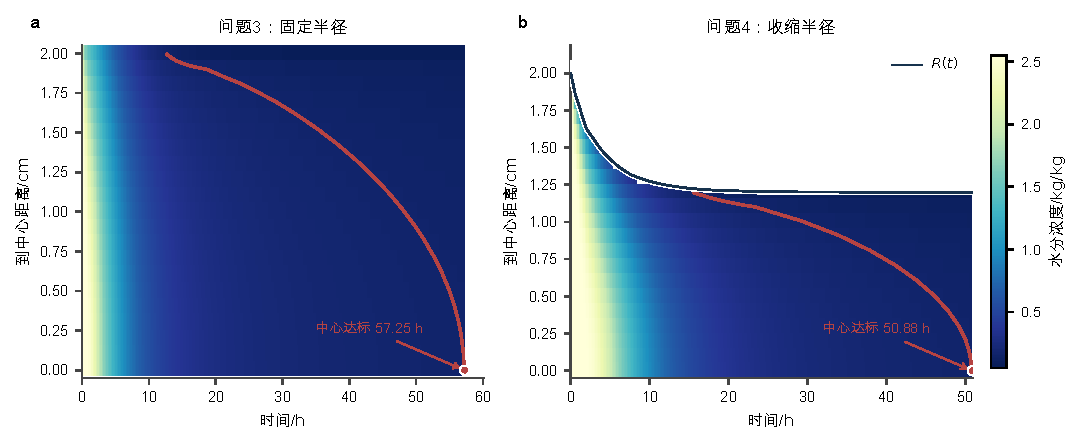
\includegraphics[width=\textwidth]{problem_a_figure_07_drying_endpoint_v03.pdf}
\caption{问题 3、4 的水分时空场。红线为 $C=0.15\unit{kg/kg}$ 的达标前沿，问题 4 的深色边界为实测半径路径 $R(t)$；两问物性不同，终点差异不能解释为纯收缩效应。}
\label{fig:endpoint}
\end{figure}

\begin{table}[H]
\centering
\caption{考虑收缩时的水分浓度（$\mathrm{kg/kg}$）}
\label{tab:q4}
\small
\begin{tabular}{rrrrrr}
\toprule
时间/$\mathrm{h}$ & $0\unit{cm}$ & $0.5\unit{cm}$ & $1.0\unit{cm}$ & $1.5\unit{cm}$ & 药材表面 \\
\midrule
6  & 1.7172 & 1.5357 & 1.0217 & -- & 0.4217 \\
12 & 0.7343 & 0.6518 & 0.4069 & -- & 0.1667 \\
18 & 0.4066 & 0.3668 & 0.2388 & -- & 0.0889 \\
24 & 0.2837 & 0.2599 & 0.1783 & -- & 0.0671 \\
30 & 0.2253 & 0.2085 & 0.1488 & -- & 0.0593 \\
36 & 0.1921 & 0.1790 & 0.1313 & -- & 0.0558 \\
42 & 0.1706 & 0.1598 & 0.1196 & -- & 0.0539 \\
48 & 0.1556 & 0.1463 & 0.1113 & -- & 0.0529 \\
50.8833 & 0.1499 & 0.1412 & 0.1080 & -- & 0.0525 \\
\bottomrule
\end{tabular}
\end{table}

表\ref{tab:q4}中的“--”表示 $1.5\unit{cm}$ 已位于收缩后药材表面之外，因此该物理位置不再定义药材内部水分浓度。结果文件仍保留题目模板的固定距离列，同时增设“药材表面”列；超出瞬时半径的单元格保持空白。

\section{模型检验、反事实与灵敏度分析}

\subsection{网格收敛、平衡与物理性检查}

表\ref{tab:convergence}列出相邻两级网格的关键差异。问题 1 的截面平均量变化与表面通量时间积分之差分别为 $6.54\times10^{-7}\,^{\circ}\mathrm{C}$ 和 $5.34\times10^{-7}\unit{kg/kg}$，验证了固定域离散的通量平衡。所有正式解的水分浓度均非负，问题 1 的表面温度高于中心温度且表面水分低于中心水分，符合干燥方向。

\begin{table}[H]
\centering
\caption{网格加密检验}
\label{tab:convergence}
\small
\begin{tabularx}{\textwidth}{C{1.3cm}C{2.4cm}C{3.0cm}C{3.0cm}X}
\toprule
问题 & 网格对比 & 温度最大差/$^{\circ}\mathrm{C}$ & 水分最大差/$\mathrm{kg/kg}$ & 达标时间差/$\mathrm{h}$ \\
\midrule
1 & $1280\to2560$ & $6.95\times10^{-6}$ & $5.43\times10^{-6}$ & -- \\
2 & $640\to1280$ & $6.27\times10^{-5}$ & $9.72\times10^{-7}$ & -- \\
3 & $1280\to2560$ & -- & $4.87\times10^{-6}$ & $0.0024$ \\
4 & $1280\to2560$ & -- & $1.94\times10^{-5}$ & $0.0003$ \\
\bottomrule
\end{tabularx}
\end{table}

对问题 4 的选定等效方程，定义材料坐标积分量
\begin{equation}
I_C(t)=\int_0^1 \xi C(\xi,t)\,\dif\xi,
\qquad
\frac{\dif I_C}{\dif t}=\frac{h_m}{R(t)}[C_\infty(t)-C_s(t)].
\label{eq:q4_integral_balance}
\end{equation}
用 $60\unit{s}$ 输出作边界通量求积，相对平衡残差为 $2.11\times10^{-4}$。进一步令 $R(t)\equiv R_0$，移动域程序与固定域程序均给出 $129.0862\unit{h}$，差异为 $0\unit{s}$，说明坐标变换实现可以正确退化。这里验证的是式\eqref{eq:moving_mass}这一选定有效 PDE 的积分平衡，不等同于已经建立含孔隙率、固相速度和干物质密度的严格变形多孔介质守恒。

\subsection{事件根、步长与独立求解器复核}

表\ref{tab:eventaudit}给出两套时间离散的独立结果。BDF 计算中将相对容差由 $2\times10^{-6}$ 收紧至 $2\times10^{-8}$，同时将最大步长从 $60\unit{s}$ 缩至 $30\unit{s}$，问题 3、4 的事件根分别只改变 $1.03\unit{s}$ 和 $0.70\unit{s}$；包括较松容差在内的最大变化不超过 $4.5\unit{s}$。因此事件根定位本身已经稳定，剩余约 $0.04\sim0.05\unit{h}$ 的差异主要来自时间/空间离散方案，而不是 $60\unit{s}$ 输出点之间的插值。

\begin{table}[H]
\centering
\caption{达标事件的独立求解与容差复核（$N=640$，单位：$\mathrm{h}$）}
\label{tab:eventaudit}
\small
\begin{tabular}{lrr}
\toprule
方法 & 问题 3 & 问题 4 \\
\midrule
全隐式有限体积（队友更新基线） & 57.2108 & 50.8634 \\
BDF，$\mathrm{rtol}=2\times10^{-6}$，$\Delta t_{\max}=60\unit{s}$ & 57.1603 & 50.8241 \\
BDF，$\mathrm{rtol}=2\times10^{-7}$，$\Delta t_{\max}=60\unit{s}$ & 57.1591 & 50.8230 \\
BDF，$\mathrm{rtol}=2\times10^{-8}$，$\Delta t_{\max}=30\unit{s}$ & 57.1588 & 50.8228 \\
\bottomrule
\end{tabular}
\end{table}

\subsection{蒸发潜热的可识别性与能量审计}

若在表面建立热质严格耦合，进入药材的净热流应写成
\begin{equation}
q_{\mathrm{net}}=h(T_\infty-T_s)-L_vj_w,
\qquad
j_w=\rho_dh_m(C_s-C_\infty),
\label{eq:latent_boundary}
\end{equation}
其中 $j_w$ 的单位必须为 $\mathrm{kg/(m^2\cdot s)}$。题给水分变量 $C$ 是干基含水率，而式\eqref{eq:mass_bc}给出的只是含水率通量；若不引入 $\rho_d$，便不能与 $L_v$ 相乘得到热流。更完整的模型还需以平衡含水率或水活度建立气固两相驱动力，而不能默认空气含湿量与固体干基含水率可以直接用于相变速率。

为判断量级，本文只作不改变正式解的诊断：取典型值 $L_v=2.4\times10^6\unit{J/kg}$，并按干基定义暂以 $\rho_d=\rho(C_s)/(1+C_s)$ 换算。定义由现有水分边界隐含的潜热需求 $q_\ell^*=L_v\rho_dh_m(C_s-C_\infty)$。在问题 2 的 $1800\unit{s}$ 时刻，
\begin{equation}
q_h=152.50\unit{W/m^2},\qquad
q_\ell^*=1008.36\unit{W/m^2},\qquad
\frac{q_\ell^*}{q_h}=6.61.
\end{equation}
对应的可用温差仅为 $6.10\unit{K}$，而维持同一传质通量所需温差为 $q_\ell^*/h=40.33\unit{K}$；前 $3\unit{h}$ 内该比值最低仍为 $6.50$。图\ref{fig:latent-audit}表明，若把潜热汇直接叠加到现有能量边界，蒸发需求会持续超过对流供热。这不是潜热可以忽略的证据，而是说明题给 $h_m(C_s-C_\infty)$ 与热边界并未构成可直接联合使用的热力学闭合。若把湿基体积密度 $\rho$ 误当作 $\rho_d$，还会进一步夸大冷却幅度。

\begin{figure}[H]
\centering
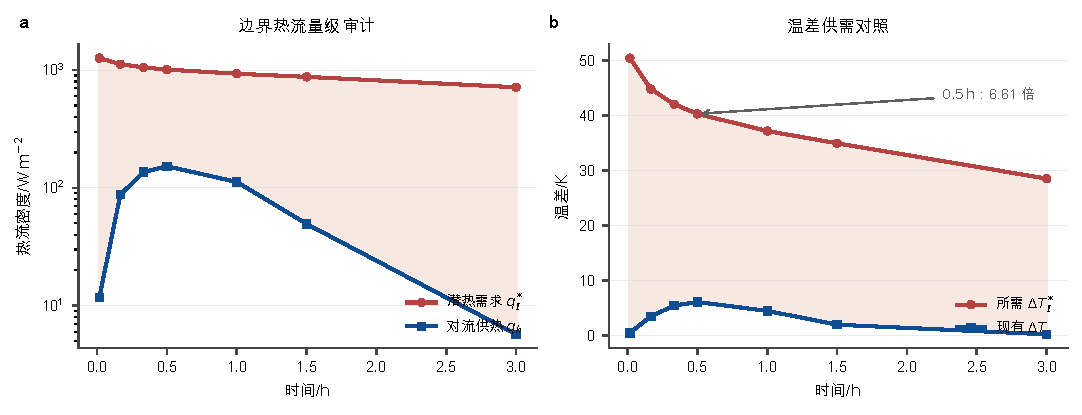
\includegraphics[width=\textwidth]{problem_a_figure_10_latent_heat_audit_v01.pdf}
\caption{蒸发潜热量级审计。红色为由现有传质边界换算的潜热需求，蓝色为现有模型的对流供热；阴影表示两者缺口。该图用于暴露闭合不足，不是潜热增强模型的预测。}
\label{fig:latent-audit}
\end{figure}

据此，正式结果保持题给解耦模型口径，不因一次不可识别的试算而改写温度场和达标时间。若获得实验数据，应同时标定 $\rho_d$、$L_v(T,C)$、平衡含水率关系和能量受限的蒸发通量，再重新求解全部温度依赖扩散系数与烘干时长。

\subsection{同物性参数下的收缩反事实}

问题 3 使用附录 3 物性，问题 4 使用附录 4 物性，直接作差会同时混入“物性关联式”和“半径路径”两种变化。为分离二者，构造 $2\times2$ 组合：每套物性分别搭配固定 $2\unit{cm}$ 半径与附件 2 收缩半径。反事实统一使用 $N=640$ 网格，仅作为稳健性证据，不替代官方高精度输出；数值见表\ref{tab:counterfactual}与图\ref{fig:counterfactual}。

\begin{table}[H]
\centering
\caption{物性关联式与半径路径的 $2\times2$ 反事实（$\mathrm{h}$）}
\label{tab:counterfactual}
\small
\begin{tabular}{lrrr}
\toprule
物性关联式 & 固定半径 & 收缩半径 & 收缩对应的时长减少率 \\
\midrule
附录 3 & 57.1589 & 25.1343 & $56.03\%$ \\
附录 4 & 129.0859 & 50.8229 & $60.63\%$ \\
\bottomrule
\end{tabular}
\end{table}

\begin{figure}[H]
\centering
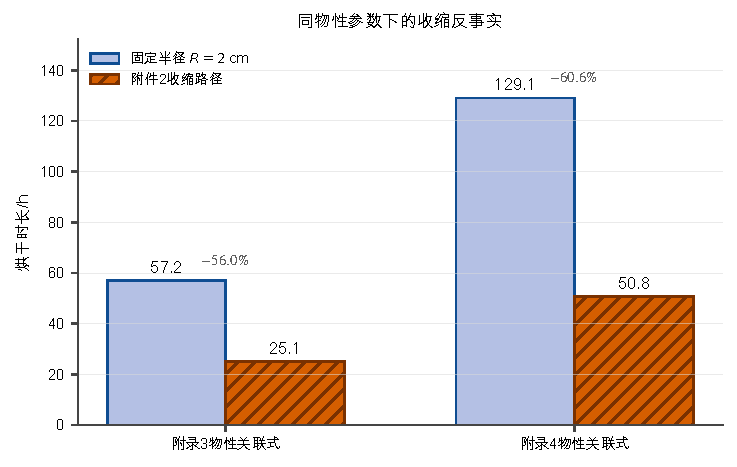
\includegraphics[width=0.72\textwidth]{problem_a_figure_08_counterfactual_v03.pdf}
\caption{同一物性关联式下的固定半径与收缩半径反事实。该差异是模型设定内的条件比较，不是实验因果效应。}
\label{fig:counterfactual}
\end{figure}

两套物性下，收缩路径均缩短模型预测时长，方向一致。这一结果说明缩短扩散距离是重要机制；但 $56.03\%$ 和 $60.63\%$ 的幅度依赖式\eqref{eq:moving_mass}的物质坐标假设，不能外推为任意药材的普遍比例。

\subsection{长期炉况、扩散关系与收缩插值的灵敏度}

附件 1 的最后一点为 $50.165\,^{\circ}\mathrm{C}$ 和 $0.04986\unit{kg/kg}$；$9000\sim14400\unit{s}$ 末段均值分别为 $50.0049\,^{\circ}\mathrm{C}$ 和 $0.049994\unit{kg/kg}$。最后一点相对均值更热约 $0.160\,^{\circ}\mathrm{C}$、更干约 $1.34\times10^{-4}\unit{kg/kg}$，故只做末值保持可能轻微缩短长期时长。表\ref{tab:extension}显示，末段均值保持和平滑渐近两种延拓均使问题 3、4 的时长增加约 $0.5\%$，方向和量级一致。因此基线结果应理解为末值延拓条件下的预测，而不是唯一工况。

\begin{table}[H]
\centering
\caption{长期炉况延拓情景（$N=640$，BDF 事件根）}
\label{tab:extension}
\small
\begin{tabular}{lrrrr}
\toprule
延拓方式 & 问题3/$\mathrm{h}$ & 变化/$\%$ & 问题4/$\mathrm{h}$ & 变化/$\%$ \\
\midrule
末值保持 & 57.1591 & 0.000 & 50.8230 & 0.000 \\
末段均值保持 & 57.4529 & 0.514 & 51.0813 & 0.508 \\
平滑渐近末段均值 & 57.4504 & 0.510 & 51.0781 & 0.502 \\
\bottomrule
\end{tabular}
\end{table}

进一步直接扰动扩散系数
\begin{equation}
D=D_0\exp\left(-\frac{a_C}{C}\right)\exp\left(-\frac{a_T}{T_K}\right).
\end{equation}
$D_0$ 改变 $\pm20\%$ 时，两问时长约变化 $-14.6\%\sim+22.2\%$；$a_C$ 改变 $\pm10\%$ 时约变化 $-20.7\%\sim+27.7\%$；$a_T$ 改变 $\pm5\%$ 时约变化 $-39.1\%\sim+72.8\%$。可见扩散关系本身远比 $h$、$h_m$ 的常规扰动更关键，尤其是 Arrhenius 指数。半径插值由分段线性改为 PCHIP 时，问题 4 时长仅变化 $-0.0069\%$，表明插值形式不是主要误差源。上述三类关键证据汇总于图\ref{fig:sensitivity}。

早期灵敏度图中“空气水分末值降低 $20\%$ 后得到 $167.24\unit{h}$”的异常分支，在 $N=1280$ 复核后变为 $57.50\unit{h}$；同时该设置改动了最后一个实测点并改变 $9000\sim14400\unit{s}$ 的插值段，并非纯粹的长期外推。故本文撤回对 $167.24\unit{h}$ 的物理解释，不再把它作为“干壳效应”证据。

\begin{figure}[H]
\centering
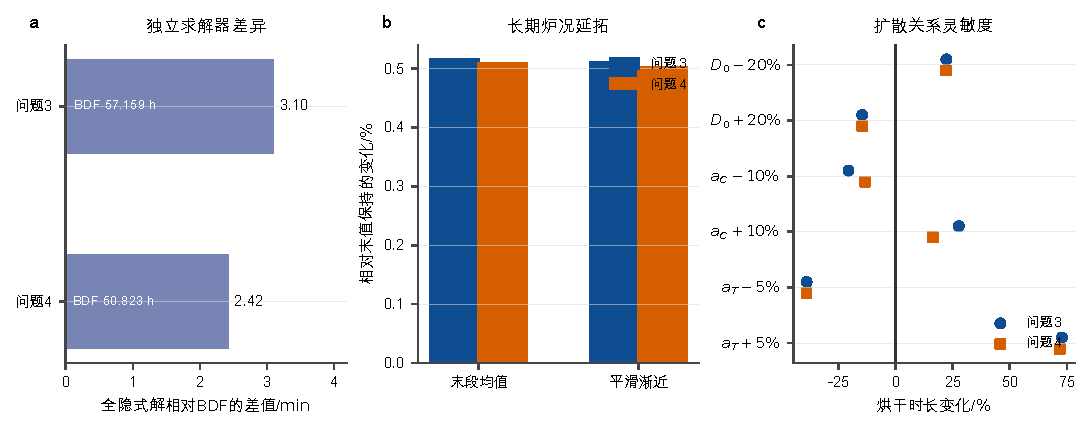
\includegraphics[width=\textwidth]{problem_a_figure_11_reviewer_robustness_v01.pdf}
\caption{关键稳健性证据闭环：独立求解器对照、长期炉况延拓以及扩散关系灵敏度。图中精确数值用于复核，正文结论按证据水平报告有效数字。}
\label{fig:sensitivity}
\end{figure}

\section{模型评价与改进方向}

\subsection{模型优点}

第一，四问共享同一有限体积框架，常物性、变物性、时变边界和收缩半径只通过参数函数替换，降低了多套程序之间的口径误差。第二，阈值事件由 BDF 根函数连续定位，提交终点同时覆盖四位小数显示误差和网格差异。第三，队友全隐式实现与 BDF 实现构成独立求解器对照，避免用单一程序自证。第四，本文没有将问题 3、4 的联合变化误判为收缩的单独贡献，而是使用同物性反事实分离半径路径效应。第五，输入检查、网格加密、有效 PDE 积分平衡、退化测试、灵敏度和 Excel 检查均纳入自动化流程；两份原始附件的哈希也已核对一致。

\subsection{模型局限}

模型的主要限制有四点。其一，一维径向近似忽略圆柱端面，中心附近的实际干燥速度可能因此偏低。其二，主能量方程没有蒸发潜热项；量级审计虽已说明机械叠加不可行，但正式温度场仍应视为题给等效热边界下的条件预测。其三，$14400\unit{s}$ 后的炉况依赖延拓，三种合理情景虽只相差约 $0.5\%$，仍缺少真正的长时实测。其四，收缩模型缺少局部速度、孔隙率和干物质密度数据，只能采用均匀物质坐标闭合；式\eqref{eq:q4_integral_balance}的通过不能替代严格的变形多孔介质守恒，反事实幅度因此具有模型依赖性。

若有进一步数据，优先开展三项改进：建立二维轴对称模型评估端部效应；以式\eqref{eq:latent_boundary}为起点联合标定能量受限的蒸发通量，而非只加一个常数潜热汇；利用多批次中心/表面含水率与半径实测数据，联合标定 $D(C,T)$、$h_m$ 和收缩速度场，并对低含水率区间单独拟合。

\section{结论}

本文建立了可覆盖四问的一维圆柱热湿传递数值模型。问题 1 在常热物性和浓度相关扩散系数下揭示了预热期的表里梯度；问题 2 的变物性结果表明温度场比水分场更快均匀。固定半径、附录 3 物性下，两套求解器支持约 $57.2\unit{h}$ 的达标时长；附录 4 物性与附件 2 收缩路径下约为 $50.9\unit{h}$。同物性反事实支持“收缩缩短扩散距离并加快模型内干燥”的机制判断，但其幅度不应脱离均匀收缩闭合作普遍推广。事件容差、长期边界延拓、有效 PDE 积分平衡和退化测试均通过相应门槛；扩散关系的指数项和潜热闭合仍是下一步实验标定的重点。

\section*{AI 工具使用声明}

本参赛队在竞赛过程中使用了AI工具，主要用于代码调试、数值结果复核、图表排版和论文语言整理，详细使用情况见支撑材料。

\begin{thebibliography}{99}
\bibitem{bergman2018} Bergman T L, Lavine A S, Incropera F P, et al. Fundamentals of Heat and Mass Transfer[M]. 8th ed. Hoboken: Wiley, 2018.
\bibitem{crank1975} Crank J. The Mathematics of Diffusion[M]. 2nd ed. Oxford: Clarendon Press, 1975.
\bibitem{patankar1980} Patankar S V. Numerical Heat Transfer and Fluid Flow[M]. New York: Hemisphere Publishing, 1980. DOI: 10.1201/9781482234213.
\bibitem{hairer1996} Hairer E, Wanner G. Solving Ordinary Differential Equations II: Stiff and Differential-Algebraic Problems[M]. 2nd ed. Berlin: Springer, 1996. DOI: 10.1007/978-3-642-05221-7.
\bibitem{virtanen2020} Virtanen P, Gommers R, Oliphant T E, et al. SciPy 1.0: fundamental algorithms for scientific computing in Python[J]. Nature Methods, 2020, 17(3): 261--272. DOI: 10.1038/s41592-019-0686-2.
\end{thebibliography}

\end{document}
